\chapter{Estat de l'art}
\label{chap:pw}

Abans d'entrar en els detalls tècnics de la implementació i funcionament d'un BMS cal conèixer el camp en qüestió. Donat que estem parlant d'un sector en evolució i on el seu mercat està en creixement, s'ha plantejat de forma hipotètica el contrast del BMS  amb els del mercat per tal de poder donar-li un valor afegit. 

S'ha fet una cerca del mercat relacionat amb els vehicles elèctrics tot buscant els aspectes que donarien viabilitat a aquest projecte tractant-lo com a producte. A més a més s'ha volgut estudiar el mercat dels VE per poder visualitzar el valor que pot tenir documentar-se en aquest tema, ja que futurament els vehicles elèctrics acabaran tenint un pes molt important, ja que la tecnologia cada dia avança més i més i tots els indicis ens indiquen que el futur seran els vehicles elèctrics.
En aquest apartat es veurà l'impacte en el mercat dels vehicles elèctrics i la viabilitat que tindria la realització del projecte en comparació amb la compra directa d'un. Cal dir que donat que el treball ha estat realitzat conjuntament amb el Marc Brunet Preses, aquesta part pot ser molt similar a la seva a nivell de documentació, ja que s'ha realitzat l'estat de l'art de forma conjunta.

\section{Mercat dels cotxes elèctrics}

A l'actualitat, l'ecologisme i l'ús d'energies sostenibles és cada cop més intens. Això ens indica que energies com l'electricitat estan agafant dia a dia una major força i per tant, tot apunta a ser un mercat que està en ple creixement. No obstant a l'actualitat, el combustible més emprat per transmetre energia a un vehicle s'extreu del petroli. El petroli és un combustible fòssil finit, i per tant, ja hi ha gent que està tenint en compte que el petroli a la llarga s'acabarà. 

Durant aquest procés d'esgotament el preu del petroli ha d'augmentar, ja que si la demanda és molt alta i la quantitat que n'existeix és molt reduïda el seu cost per força ha d'incrementar. És per això que l'impacte de vehicles elèctrics comença el seu camí per a instal·lar-se dins del mercat, ja que fa relativament poc que els vehicles elèctrics es comencen a conèixer i a manufacturar a gran escala. A més a més ja comencen a aparèixer infraestructures per a carregar aquests tipus de vehicles a les grans ciutats i per tant ja comencen a haver-hi facilitats. 
\newline
No obstant, el fet de que el petroli sigui finit no vol dir que en qüestió de 5 anys ja s'hauran esgotat totes les reserves de petroli del món, encara queden grans reserves de petroli per tot el món i les que encara no han estat trobades. La demanda del petroli segueix en augment ja que la quantitat de cotxes segueix en augment. En la següent gràfica es pot apreciar com fins l'any 2016 no ha parat de créixer la demanda del petroli:
\bigskip

\begin{figure}[H]
		\centering
    	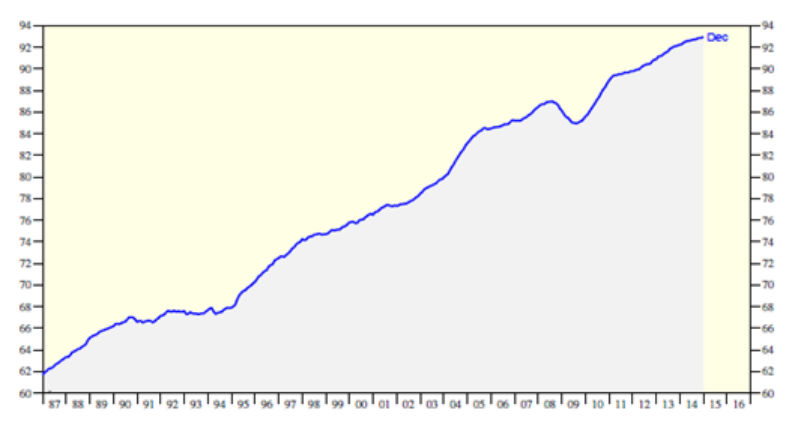
\includegraphics[width=\textwidth]{Marcteoric/Augmentdemandapetroli.png}
     	\caption{Demanda mundial de petroli, valor mig per any}
\end{figure}

En les grans ciutats ja comencen a aparèixer polítiques que prohibeixen l'entrada a vehicles que superen un cert grau de contaminació, ja que l'acumulació d'aquest pot pujar els nivells de contaminació de la ciutat per sobre del que regeix la llei. Els vehicles elèctrics no contaminen \newline pràcticament res, si no tenim en compte el seu procés de fabricació. Els vehicles híbrids funcionen amb electricitat fins que el motor ja ha de donar una certa potència, això ja suposa que el vehicle ha d'anar a una gran velocitat, fora de les velocitats màximes permeses en una zona urbanitzada. A més a més, el preu de la gasolina és molt elevat comparat amb el de l'electricitat. 

El preu d'un vehicle de combustió o un vehicle que funciona amb electricitat no és tant distant, no estem parlant que un cotxe elèctric pugui arribar a costar el doble d'un de gasolina, els preus es troben bastant parells, tot i que encara són més econòmics els de combustió. Es preveu que per al 2022 el cost total sense subsidi per als propietaris de bateria caurà per sota de la d'un vehicle de combustió. 

Per tots aquests motius i els preus assequibles dels vehicles elèctrics, el mercat dels VE es troba en augment. La previsió per als següents anys és que la demanda creixerà de forma exponencial. Al 2040 es preveu que els vehicles elèctrics seran un 35\% de les ventes mundials d'automòbils.

\begin{figure}[H]
		\centering
    	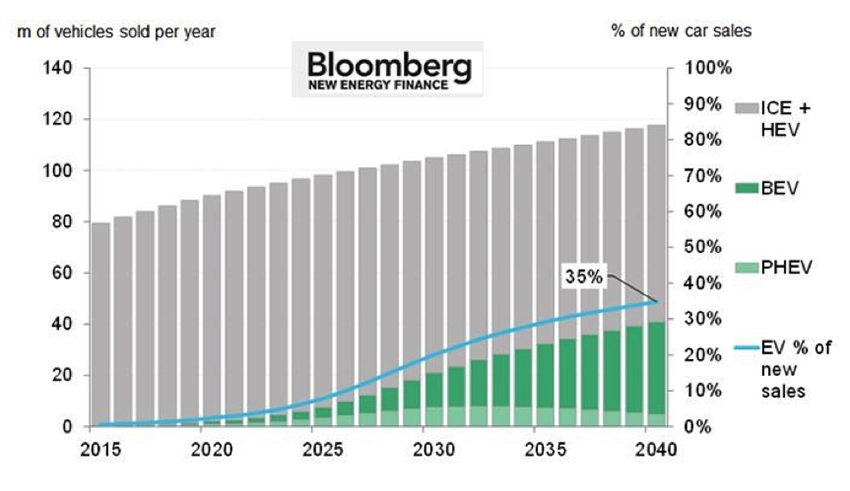
\includegraphics[width=\textwidth]{Marcteoric/ev-sales-distrib.png}
     	\caption{Previsió d'increment de la venda de vehicles elèctrics.}
\end{figure}

A la figura 2.2 es mostra de forma detallada la previsió de l'evolució del mercat dels vehicles. En primer lloc tindríem els ICE + HEV. Aquests vindrien a ser els vehicles que funcionen per combustió (dièsel/gasolina) i els híbrids que també fan servir la combustió. Es pot veure com són els que lideren encara el mercat, tot indicant que el petroli seguirà sent la font d'energia principal per als vehicles en general. 

En segon lloc tindríem els BEV(Battery Electric Vehicle) que són els vehicles que funcionen mitjançant bateries. Aquests assoliran un 30\% \newline d'increment l'any 2040. Per qüestions ecològiques que podrien succeir en el futur aquest valor pot decréixer considerablement si s'estableixen límits de contaminació molt baixos. Les subvencions de l'estat per als vehicles elèctrics també podria girar la balança i que agafessin en el futur un major pes.
 

En última instància hi ha els PHEV ( Plug-In Hybrid Electric Vechicle) que són els vehicles híbrids endollables a la corrent. Encara és incert el futur d'aquest tipus de vehicles i per això no hi ha gran confiança en aquests.

\section{Mercat dels vehicles elèctrics (no cotxes)}

Tot i que el món dels vehicles elèctrics està totalment centrat en els cotxes, també existeixen altres vehicles que fan servir l'electricitat com a font \newline d'energia. El controlador que es plantejarà en tot aquest projecte està pensat molt més per a aquest tipus de vehicles que no pas per a cotxes. Entre aquests vehicles podríem trobar el patinet elèctric, Hoverboard i la bicicleta elèctrica entre d'altres. No només això sinó que també el nostre controlador pot estar emprat per a vehicles dedicats a persones amb mobilitat reduïda com podria ser una cadira de rodes elèctrica o els típics "tricicles" que fa servir la gent gran. Per últim caldria posar els vehicles radiocontrol(RC), des de llanxes fins avions. 

Per a la majoria de vehicles esmentats no és precís aconseguir carnet de conduir o bé una llicència ni assegurança, però ve cal conèixer la normativa que regula l'ús d'aquests vehicles en llocs urbans. Cada municipi té els seus permisos i prohibicions. La normativa pot canviar depenent del pes o bé la velocitat màxima. Per això s'aconsella informar-se sobre la legislació del seu ajuntament. Sobretot a les grans ciutats és on la legislació és més estricta. Un exemple d'aquest podria ser la legislació actual de Barcelona sobre els patinets elèctrics. Els patinets elèctrics conformen els vehicles elèctrics de Tipus B.

\begin{figure}[H]
		\centering
    	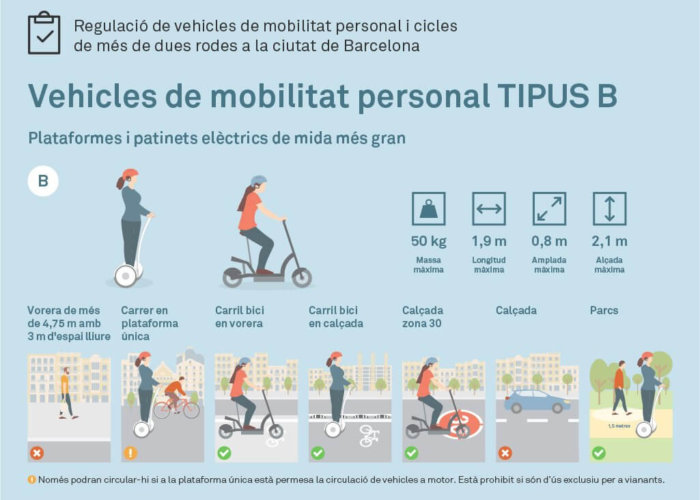
\includegraphics[width=12cm, height=7cm]{Marcteoric/normativaBCNpatinetselectrics.jpg}
    	\caption{Normativa de vehicles tipus B a Barcelona.}
\end{figure}

Si es parla de l'autonomia dels altres vehicles elèctrics no s'apropa ni de bon tros a l'autonomia d'un cotxe elèctric. Les autonomies d'aquests tipus de vehicles poden arribar als 40 minuts aproximadament, sent la bicicleta qui té una major autonomia. Depenent de la potència del motor, de la capacitat de la bateria i també com es condueixi aquest vehicle aquest temps pot variar. Un bon manteniment de la bateria també suposa una major durabilitat en l'autonomia. Ara es mostraran alguns vehicles elèctrics que són els que tenen un impacte més gran al mercat.

\subsection{Patinet elèctric}
El patinet elèctric és una opció alternativa de transport ecològic per circular a nivell econòmic sense gastar res en gasolina. Són sustentables, lleugers, pràctics i ràpids. Són útils tant per aquelles persones amb mobilitat reduïda, com per estudiants, treballadors i persones amb l'objectiu de desplaçar-se d'una forma senzilla d'un lloc a un altre en un curt període de temps, estalviant gasolina i transport públic.

L'enorme majoria dels patinets tenen un motor anomenat Brush (amb escombretes de llarga durada), de gama econòmica. Els patinets elèctrics dissenyat per la conducció del peu, on el seu diàmetre de roda és més gran, disposen d'un altre gènere de motor anomenat Brushless, que vindria a fer el mateix que el motor Brush, però sense escombretes. 

L'autonomia del patinet elèctric és la combinació de múltiples factors: La capacitat de la bateria (Volts i Amperes), la potència del motor (Watts), càrrega del patinet elèctric (massa pròpia), càrrega (massa conductor), inclinació del terreny i velocitat.
En línies generals, un patinet elèctric acostuma a tenir una autonomia d'entre 40 minuts en models de 800W a 55-60 minuts en els models de 1000-1500W.
\bigskip

\newpage 
\subsubsection{Xiaomi Mi Scooter}  
El Xiaomi Mi és el patinet elèctrics més venguts a la web d'Amazon. Està pensat per a una persona de fins a 75Kg. Té un abast de fins a 30Km amb una sola càrrega. Pot arribar a velocitats de fins a 35Km/h. El seu preu ronda els 380€. 
\begin{figure}[H]
		\centering
    	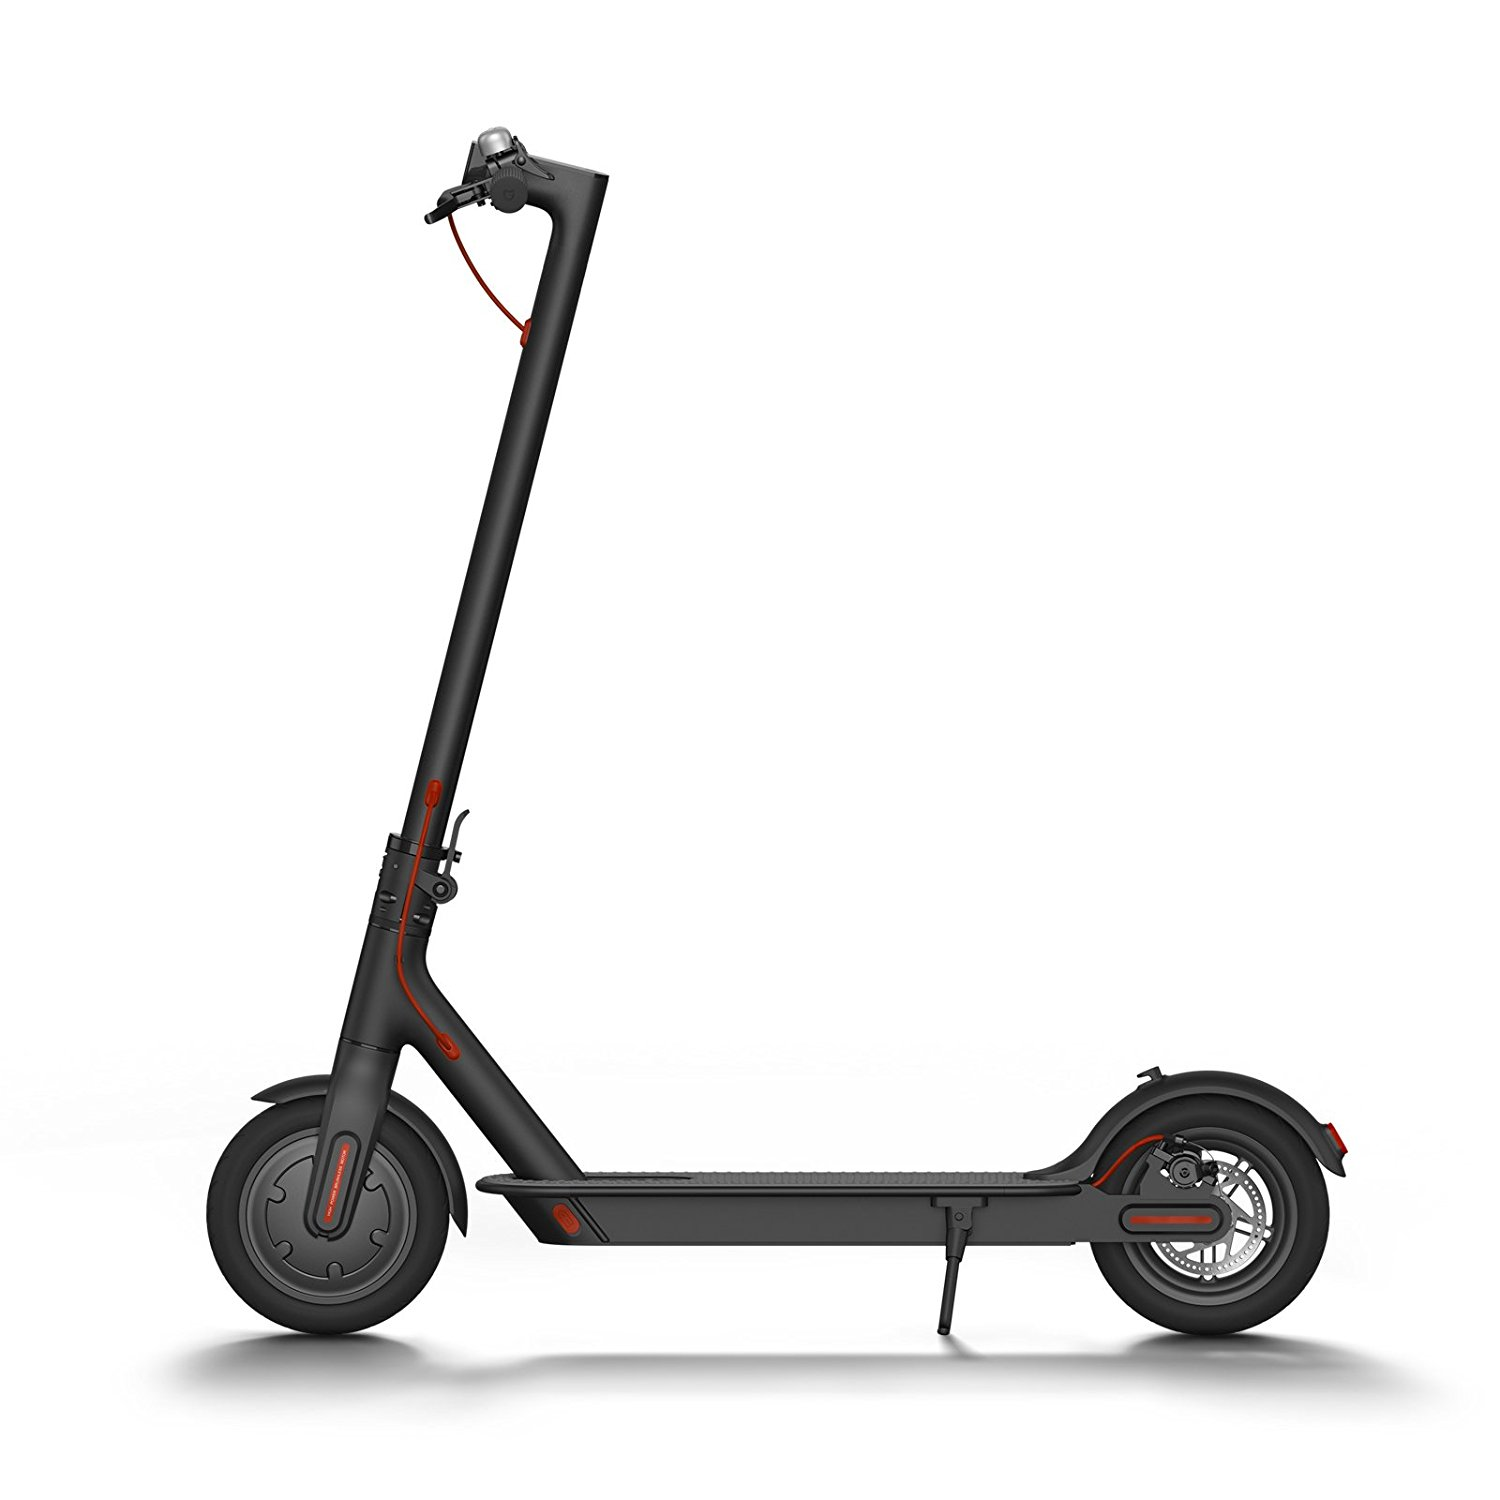
\includegraphics[width=10cm, height=10cm]{Marcteoric/patinetelectricxiamoi.jpg}
     	\caption{Xiaomi Mi Scooter.}
\end{figure}

\subsubsection{Homcom Patinet elèctric} 
El Homcom és un patinet plegable elèctric tipus Scooter, aquest model es trobaria a la gama baixa de patinets elèctrics. Està pensat per a una persona de fins a 50Kg. Té un abast d'entre 10-15Km amb una càrrega sencera. Pot arribar a una velocitat de fins a 12Km/h. El seu preu ronda els 100€.
\begin{figure}[H]
		\centering
    	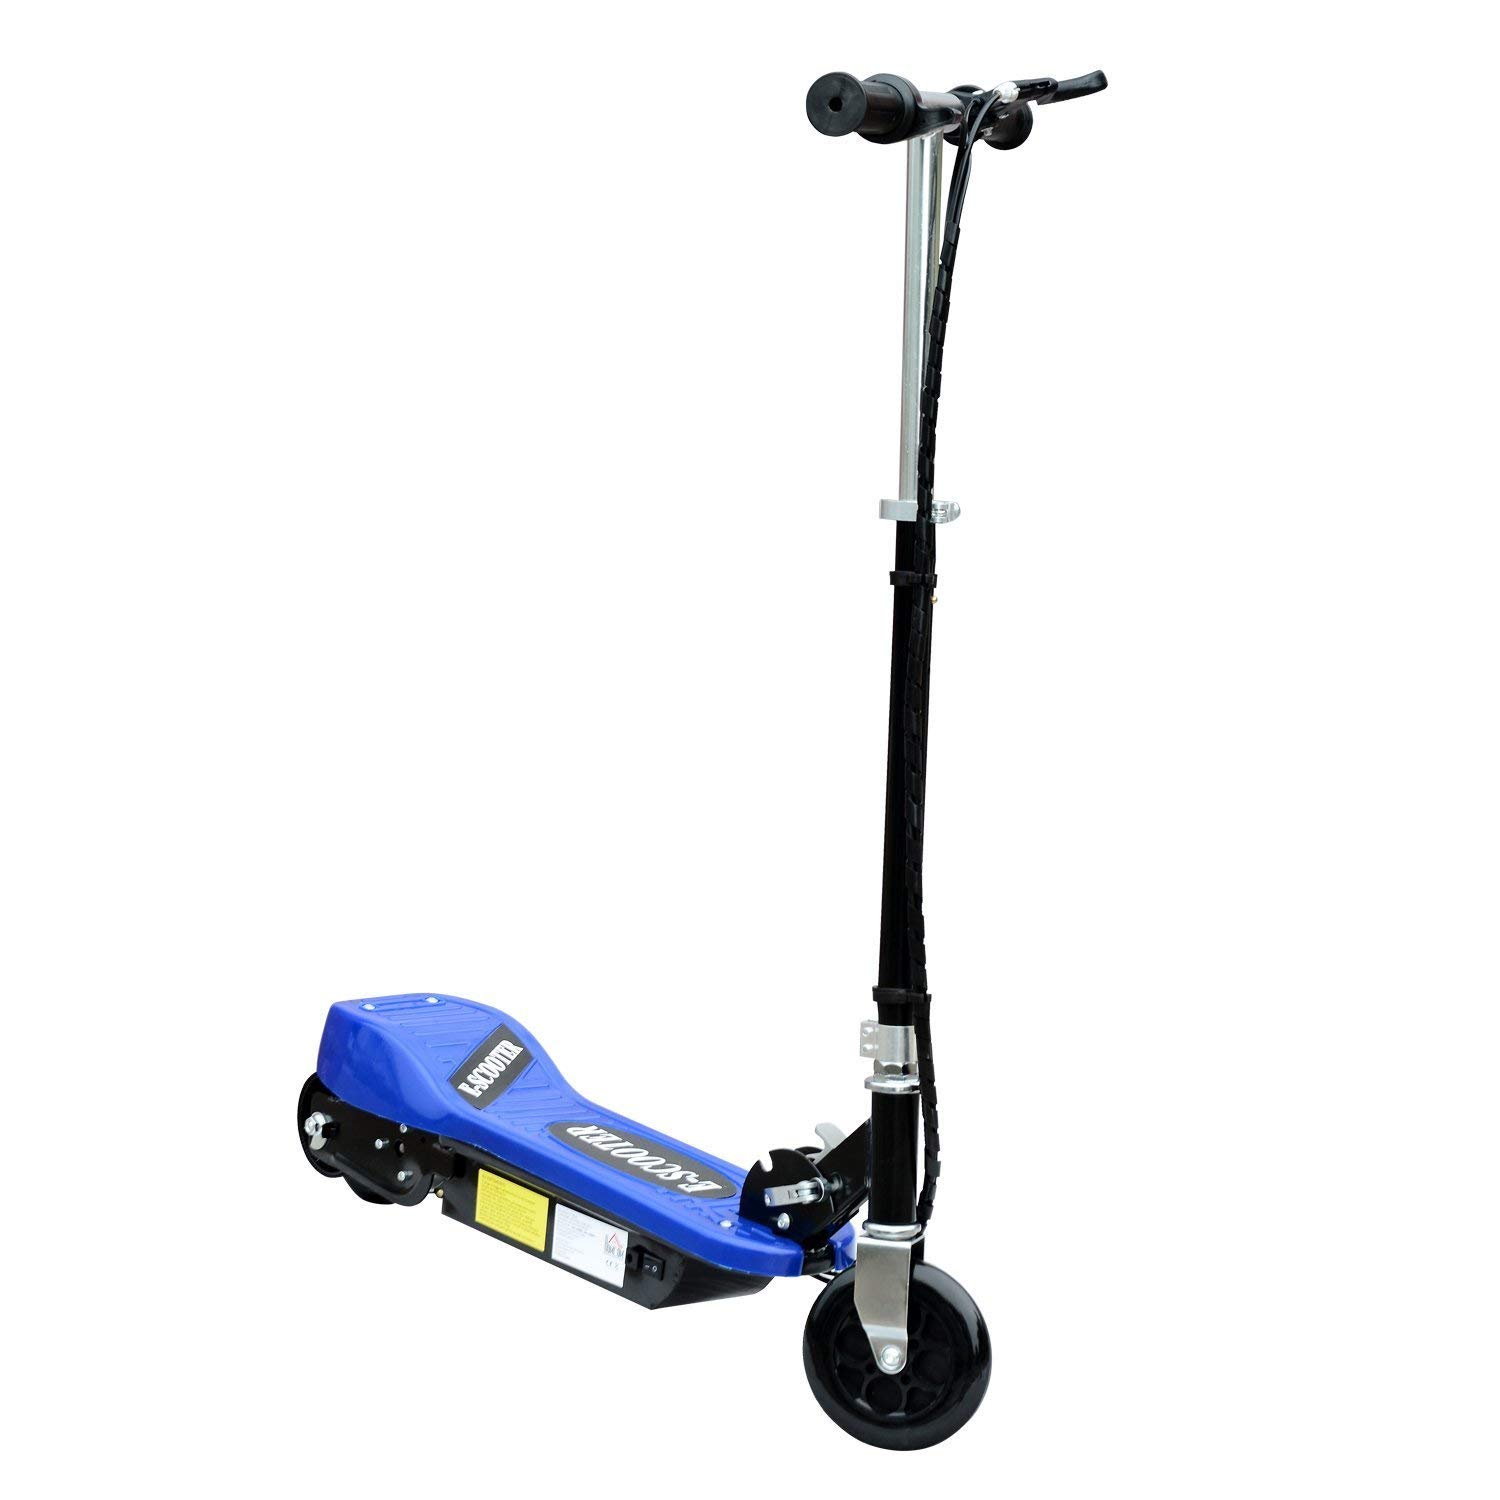
\includegraphics[width=8cm, height=8cm]{Marcteoric/Homcompatinetelectric.jpg}
     	\caption{Homcom patinet elèctric}
\end{figure}

\subsection{Hoverboard}
Aquests patinets han aparegut fa poc temps. Són únics en la forma en la que funcionen ja que s'autoequilibren, de tal forma que l'usuari pot accelerar i frenar tan sols movent el seu cos cap endavant o cap enrere. De la mateixa manera, girar és tan senzill com inclinar lleugerament el cos cap a un costat o l'altre. El funcionament d'aquest patinet es basa en el funcionament de diferents mecanismes. En primer lloc, les bateries es connecten a dos motors elèctrics independents en cada roda. Per altra banda, es troba el component més important per a mantenir l'equilibri, el giroscopi. Aquest detecta quan canvia d'orientació el patinet per a, d'aquesta forma, poder mantenir l'orientació adequada. 

El giroscopi funciona mitjançant un sensor magnètic que detecta la direcció de moviment i la velocitat rotacional de la roda. 
Tot el sistema es troba connectat a una unitat central de processament (CPU). El giroscopi mesura constantment l'orientació de la roda, i envia un senyal a la CPU per a que es processi e interpreti. D'aquesta forma, si el patinet s'inclina cap endavant s'envia l'ordre d'accelerar els motors per a compensar aquesta inclinació. Pel contrari, si s'inclina cap enrere es produirà l'efecte invers. Ara es mostraran dos exemples per veure com estan implantats aquests productes al mercat. \newline \bigskip

\subsubsection{Hooboard} 
El Hooboard és un Hoverboard de gama alta. Té una autonomia de fins a 15Km i una velocitat màxima de fins a 15Km/h. Està composat per dos motors de 400W i el seu preu ronda els 500€.
\begin{figure}[H]
		\centering
    	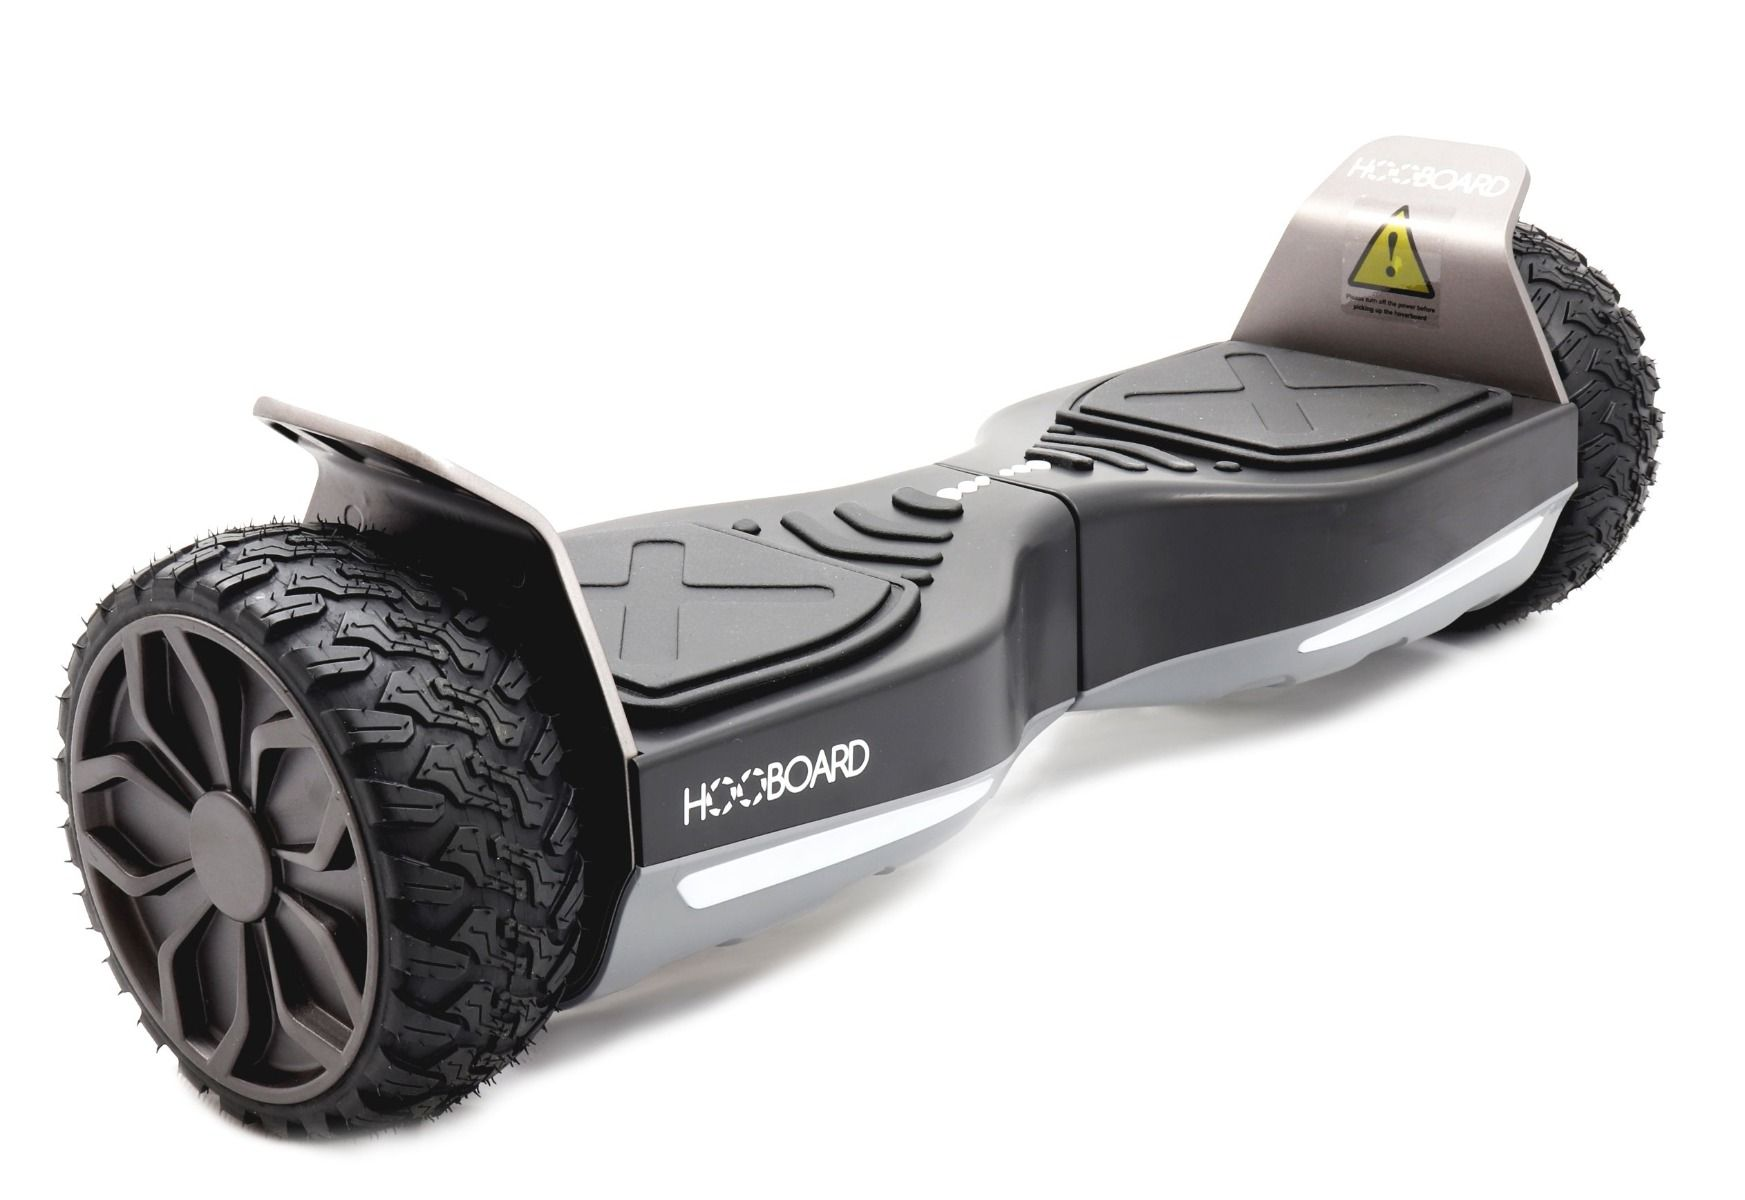
\includegraphics[width=7cm, height=5cm]{Marcteoric/hooboard.jpg}
     	\caption{Hooboard}
\end{figure}


\subsubsection{BEBK Hooverboard} 
El BEBK Hooverboard és un Hooverboard que funciona mitjançant motors elèctrics Brushless. Consta de dos motors de 350W. Pot arribar a velocitats de fins a 12Km/h i una autonomia de fins a 18Km. El seu preu ronda els 150€.
\begin{figure}[H]
		\centering
    	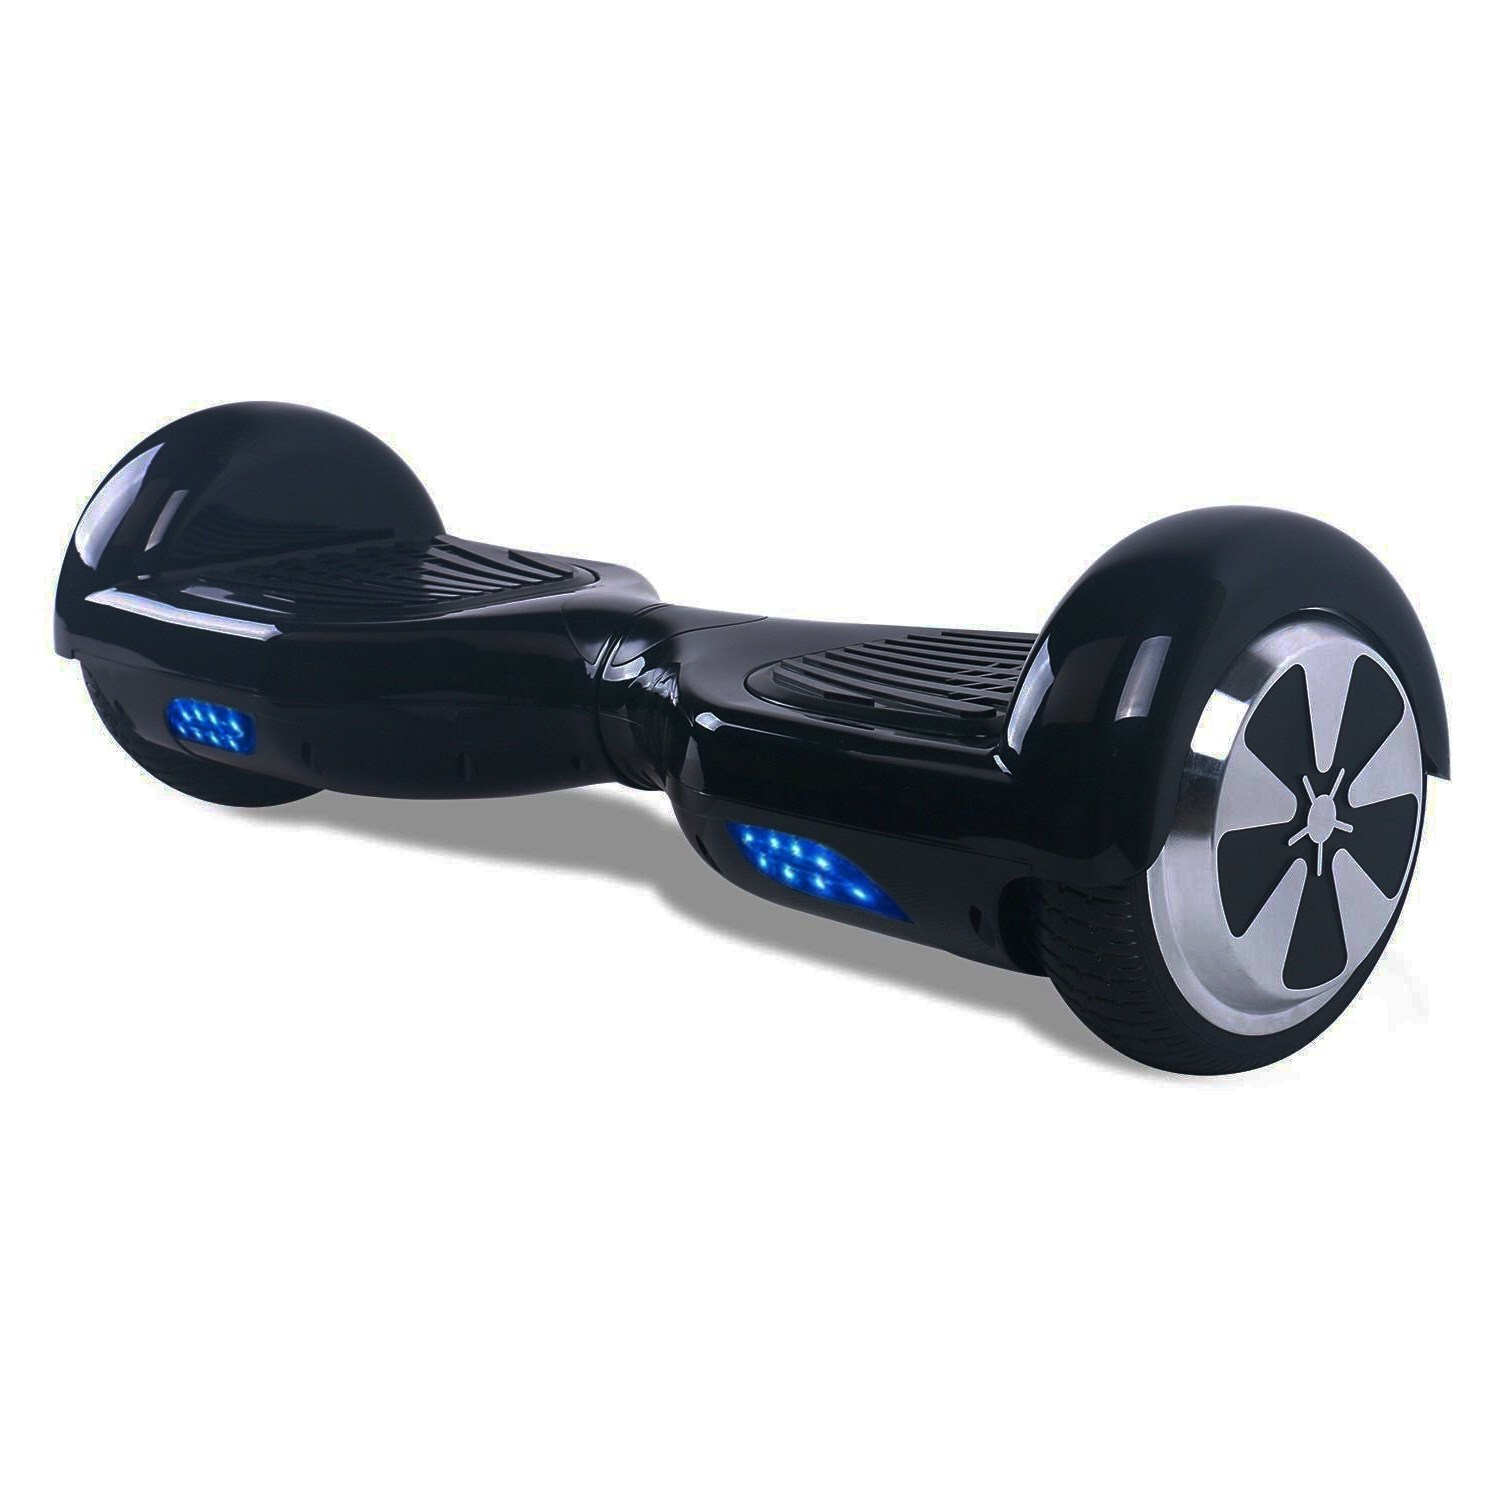
\includegraphics[width=7cm, height=7cm]{Marcteoric/bebkhooverboard.jpg}
     	\caption{BEBK Hooverboard}
\end{figure}

\subsection{Bicicleta elèctrica}
Al 2016 les ventes de bicicletes elèctriques van arribar, en tot el món, a uns 35 milions d'unitats. La millora de la tecnologia de les bateries d'ions de liti està donant com a conseqüència bicicletes elèctriques més lleugeres, més econòmiques i cada cop més similars a les bicicletes tradicionals.

Les altes tasses d'urbanització, la millora de la tecnologia de les bateries i els components de les bicicletes, les polítiques locals relacionades amb la contaminació, el desig creixent d'abandonar modes de transport motoritzats, el seu major rendiment i baix cost impulsen la indústria de la bicicleta elèctrica. Les bicicletes elèctriques es troben situades en una posició ideal per a ser les majors beneficiades d'aquesta tendència de canvi, pel seu baix cost en relació amb l'automòbil, per no requerir carnet pel seu maneig i per l'existència, cada cop en major mesura d'infraestructures especialment dedicades a elles. \newline \bigskip

             
\subsubsection{Extrbici XF800 Electric ATV } 
L'Extrbici XF800 Electric ATV és una bicicleta elèctrica que pot portar una càrrega de fins a 160Kg, pot arribar a 50Km/h amb una autonomia relativa de fins a 80Km. El seu preu rondaria els 1900€
\begin{figure}[H]
		\centering
    	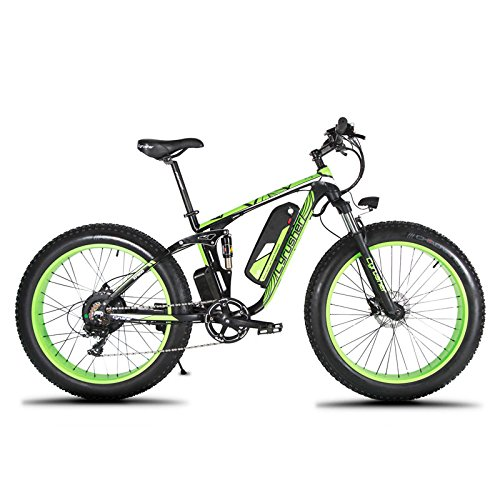
\includegraphics[width=8cm, height=8cm]{Marcteoric/extrbicixf800electricatv.jpg}
     	\caption{Extrbici XF800 Electric ATV}
\end{figure}
                      
\subsubsection{FOLLOW UP E05 }
El FOLLOW UP E05 és una bicicleta elèctrica que pot portar una càrrega de fins a 100Kg, pot arribar a 22Km/h amb una autonomia de fins a 30Km. Funciona amb motor Brushless de 250W i el seu preu ronda els 400€.
\begin{figure}[H]
		\centering
    	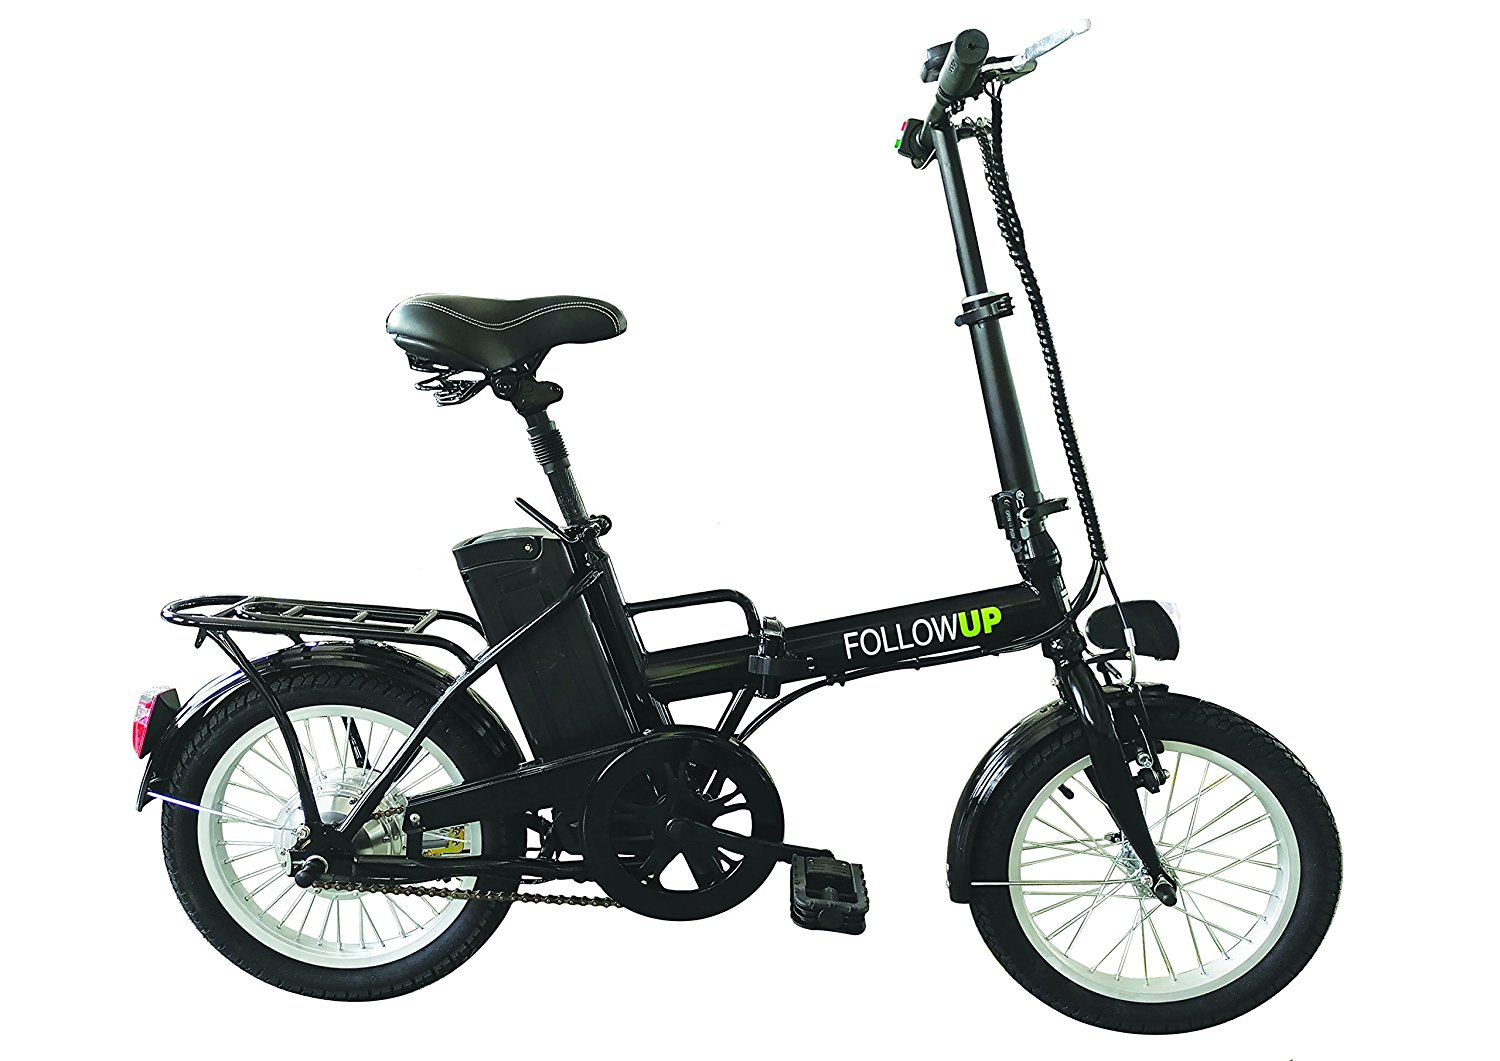
\includegraphics[width=10cm, height=7cm]{Marcteoric/followupe05.jpg}
     	\caption{FOLLOW UP E05}
\end{figure}

\section {Mercat de les bateries emprades per als VE}
Les bateries d'ions de liti ja formen part de la vida quotidiana i estan incloses en telèfons mòbils, tauletes i raspalls de dents elèctrics, entre d'altres aplicacions. En els últims anys s'han produït diferents avenços tecnològics en aquest tipus de bateries per a poder ser emprades en els vehicles elèctrics. Encara que l'adopció dels vehicles elèctrics no estigui sent tan positiva com s'esperava, les bateries ja suposen un component cada cop més rellevant dins de la indústria automobilística. Donat que les bateries són una part significativa dels costos d'un vehicle elèctric, existeixen considerables incentius per augmentar l'eficiència dels seus processos de producció, reduir els seus costos i millorar el seu rendiment. El sistema elèctric es beneficiarà del desenvolupament d'aquestes bateries, al construir una solució per emmagatzemament de l'energia generada per les tecnologies renovables intermitents, que permetran reforçar la seva seguretat de subministrament.

Respecte als reptes que té aquesta tecnologia a superar, cal destacar la falta d'una única tecnologia d'emmagatzemament que sigui capaç de cobrir totes les necessitats del mercat. Això provocarà que el sistema pugui contemplar la incorporació de diferents tipus de bateries. 

Addicionalment, a l'igual que qualsevol altre component del sistema elèc- \newline tric, els sistemes de gestió de bateries hauran de lidiar amb els possibles atacs tecnològics que puguin sofrir. En definitiva, el desenvolupament dels vehicles elèctrics permetrà avançar en les tecnologies de bateries \newline d'emmagatzemament. Les bateries hauran de considerar-se com a part de l'estratègia de les energies renovables, contribuint a arribar a un sistema energètic més eficient.

\subsection{Previsió de mercat per al futur de les bateries}

Com ja s'ha comentat prèviament, les bateries jugaran un paper molt important dintre dels vehicles elèctrics. Això vol dir que ja s'implementen estratègies per tal d'optimitzar el màxim els costos i rendiment d'aquestes. A la dècada del 2030 podríem estar parlant que el preu de baixada respecte el 2010, que és quan van començar a aparèixer de forma global les bateries d'ió-liti, estaria suposant aproximadament una reducció de cost de fins al 75\%. No només es reduiran els preus de les bateries, sinó que la compra \newline d'aquestes bateries augmentarà considerablement en els últims anys arribant a valors que superin els catorze mil milions de dòlars l'any 2026.
\begin{figure}[H]
		\centering
    	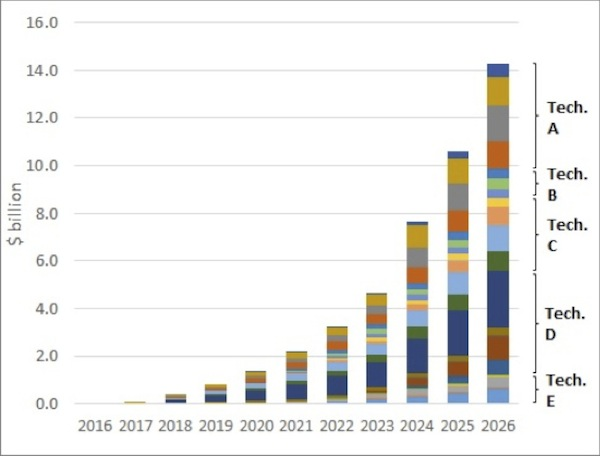
\includegraphics[width=13cm, height=8cm]{Marcteoric/ventabateries2026.jpg}
     	\caption{Previsió de ventes de bateries en funció del tipus de vehicle.} 
\end{figure}

\subsection{L'hora de l'economia del liti}
Les bateries de liti estan totalment consolidades a la vida quotidiana. Són necessàries per alimentar des de petits dispositius fins a sofisticats vehicles elèctrics. La previsió és que el seu consum augmenti en els pròxims anys, especialment fomentat per l'auge de l'Internet de les Coses i altres aplicacions tecnològiques.

Degut a la predicció del decreixement del cost d'aquest tipus de bateries s'està impulsant de forma massiva aquest mercat. Aquesta caiguda de preus és probable que provingui d'un augment de la demanda degut a la propagació dels cotxes elèctrics, que està permetent als fabricants augmentar la producció. 
\begin{figure}[H]
		\centering
    	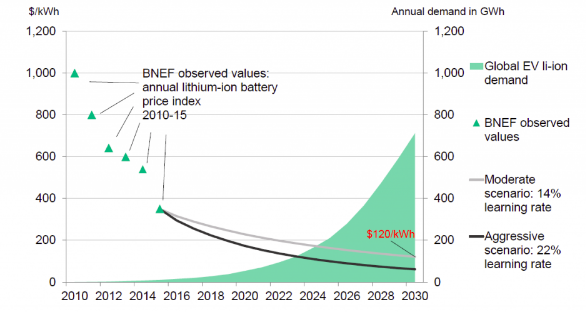
\includegraphics[width=13cm, height=8cm]{Marcteoric/mercatbaterialitioion.png}
     	\caption{Previsió del mercat de les bateries d'ions del liti.} 
\end{figure}

\section{Recerca de gestors de bateries al mercat}
Al mercat actual no existeixen controladors de vehicles totals, és a dir, un controlador que s'encarregui de tot el procés de control de la bateria fins al control del motor. Al mercat queda diferenciat en aquests dos grans blocs que normalment són compatibles entre ells. És per això que cal buscar per separat els gestors de bateries i els drivers del motor. Com el meu projecte va enfocat als BMS exposaré un exemple per després contrastar-ho amb la nostra idea de prototip. El BMS que es mostrarà a continuació es l'Orion BMS.

\subsection{Orion BMS}
Si es busca un BMS de confiança per a gestionar bateries de liti l'Orion BMS és una opció a tenir molt en compte. És un molt bon gestor de bateries altament valorat en el mercat. La seva fiabilitat i totes les seves característiques fan que sigui un BMS de molt alta gama. Compta amb una interfície per a que l'usuari el pugui configurar. Pot controlar des de 24 fins a 180 cel·les i el seu preu es troba entre els 1,000\$ i els 2,300\$.

Les seves característiques elèctriques serien les següents:

\begin{figure}[H]
		\centering
    	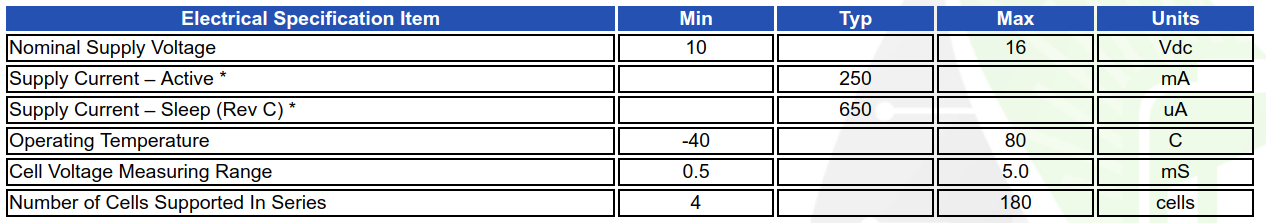
\includegraphics[width=\textwidth]{Marcteoric/electricalspecsorionbms.png}
     	\caption{Característiques elèctriques de l'OrionBMS.}
\end{figure}

Les seves especificacions generals serien les següents:

\begin{figure}[H]
		\centering
    	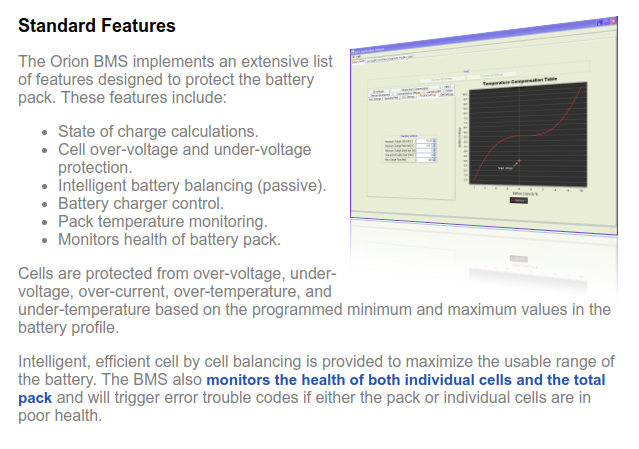
\includegraphics[width=12cm,height=5.5cm]{Marcteoric/stdftsorionbms.png}
     	\caption{Especificacions generals de l'OrionBMS.}
\end{figure}

La seva interfície per a l'usuari és la següent:

\begin{figure}[H]
		\centering
    	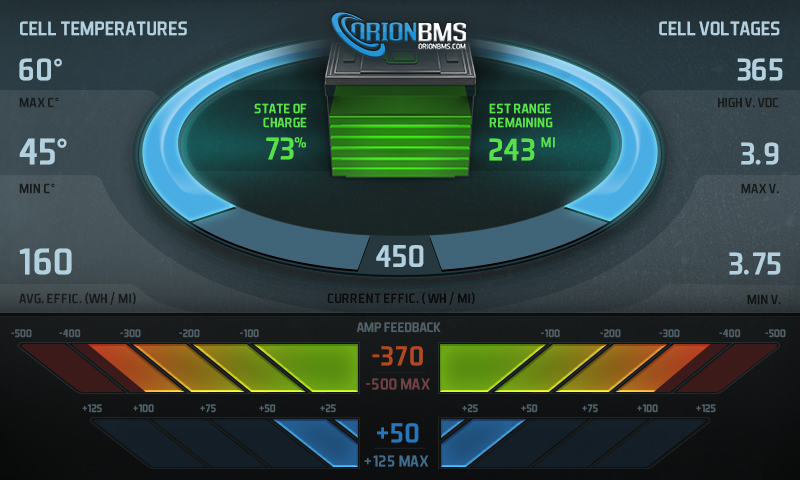
\includegraphics[width=\textwidth,height=7cm]{Marcteoric/orionbmsinterface.jpg}
     	\caption{Interfície de l'OrionBMS per a l'usuari.}
\end{figure}

No es vol entrar molt en detall ja que aquests fabricants tenen protocols privatius els quals no indiquen com realitzen per exemple l'estimació del SOC, un dels principals paràmetres a tenir en compte en un BMS. Sent tot privat és molt complicat contrastar-ho a nivell tècnic.

Els comentaris respecte aquest BMS són molt positius, però tenim encara la qüestió de que són encara molt cars. Si el nostre BMS l'aconseguim realitzar podríem estar competint a nivell de preu de venta, pensant en el nostre projecte com a producte. Si només el contemplem com un projecte per a nosaltres per aconseguir gestionar correctament una bateria, el preu disminuiria altament, per tant a nivell de preu estem en una molt bona posició.

\section{Recerca de projectes de codi obert de BMS}

Existeixen molts projectes de codi obert basats en gestors de bateries. Uns només mostren el software i altres només donen el hardware. És molt complicat doncs implementar un BMS en la seva totalitat en projectes de petita escala. No obstant, hi ha un projecte que s'ha diferenciat de la resta per ser un dels més complexes. Aquest projecte s'anomena Fox BMS.

\subsection{Fox BMS}
Avui en dia existeix un dels projectes més grans d'un disseny de BMS de codi lliure anomenat Fox BMS. És gratuït, obert i flexible per a entorns de recerca i desenvolupament per al disseny de BMS. La part més increïble és que és la primera empresa que dóna en la seva totalitat tant la part de hardware com la part de software. El fet d'oferir tot el projecte a la comunitat ha fet que la pròpia comunitat hagi desenvolupat encara més aquest projecte. Aquesta comunitat no està només composada per petites comunitats de gent, o individus, sinó que també grans empreses han participat en aquest projecte. El fet de que les grans empreses hagin participat en aquest projecte ha sigut el punt clau per a que aquest projecte sigui mundialment conegut en l'entorn de les bateries.

Els creadors d'aquest BMS han desenvolupat fins i tot un vehicle elèctric, obert al mercat, que funciona amb aquest gestor de bateries. L'estructura complerta d'aquest projecte es mostra a la següent figura:

\begin{figure}[H]
		\centering
   	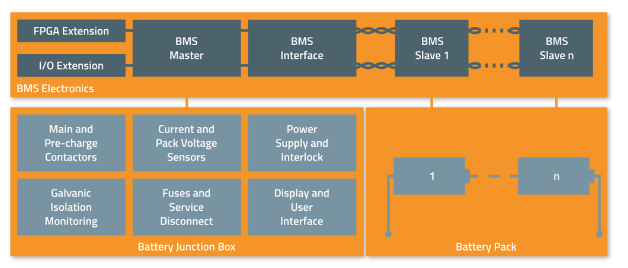
\includegraphics[width=\textwidth, height=6cm]{Marcteoric/estructurafoxbms.png}
     	\caption{Arquitectura del FOX BMS.} 
\end{figure}

El FOX BMS és un BMS modular de desenvolupament, amb l'objectiu de controlar les bateries per a l'automoció, l'aviació, l'espai, vaixells, trens, bateries industrials i per a energies renovables. És un projecte que està sempre en desenvolupament. Totes les característiques que dóna aquest BMS queden reflectides en la següent figura:

\begin{figure}[H]
		\centering
   	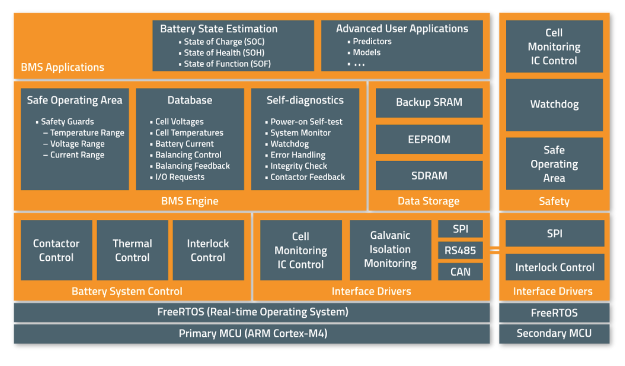
\includegraphics[width=\textwidth, height=6cm]{Marcteoric/aplicacionesfoxbms.png}
     	\caption{Característiques del FOX BMS.} 
\end{figure}

Les funcions principals d'aquest BMS són compartides amb la majoria de BMS del mercat. Bàsicament és poder fer l'estimació tant del SOC com del SOH, que és principalment el control constant de les cel·les per assegurar que funcionen correctament. També controlen la temperatura de les cel·les. No obstant, aquest projecte compta amb moltes més característiques que fan que sigui un dels BMS més potents del mercat. \newline D'aquestes característiques destaquen tant el monitoreig constant de les cel·les com algorismes que prediuen aspectes futurs que poden succeir a les cel·les. D'aquesta manera el sistema queda molt més robust ja que prediu els possibles errors amb un cert marge de temps, suficient com per evitar problemes. 
\bigskip
\begin{figure}[H]
		\centering
   	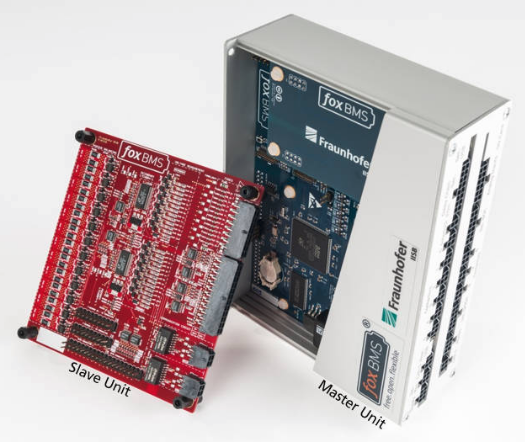
\includegraphics[width=8cm, height=7cm]{Marcteoric/foxbmsimatge.png}
     	\caption{Model de venta del FOX BMS.} 
\end{figure}

Aquest projecte és massa complex per a una persona que comença a \newline conèixer el món dels gestors de bateries. És per això que només s'han esmentat els seus aspectes principals. 

\section{Marc del projecte}
Per desenvolupar un BMS cal conèixer en primer lloc quines bateries existeixen i quines són les seves característiques principals. Això quedarà explicat en el següent capítol del projecte, en l'apartat de bateries. Un cop vistes les diferents bateries es procedirà a fer l'elecció d'un tipus d'aquestes, el qual servirà de base per a la implementació del BMS. És a dir, que el BMS es realitzarà en funció del tipus de bateria que s'esculli. Un cop escollida la bateria es tornarà a indagar sobre els diferents conceptes amb els quals treballa un BMS i finalment es procedirà en la implementació teòrica d'un BMS. Aquest integrat quedarà representat de forma esquemàtica amb \newline l'electrònica mínima que requereix per a veure la implementació d'aquest. 
